\section{APPLICATION: DEMAND RESPONSE}
\label{S:casestudy}

In January 2014, the east coast (PJM) electricity grid experienced an 86x increase in the price of electricity from \$31/MWh to \$2,680/MWh in a matter of 10 minutes. Similarly, the price spiked 32x from an average of \$25/MWh to \$800/MWh in July of 2015. This extreme price volatility has become the new norm in our electric grids. Building additional peak generation capacity is not environmentally or economically sustainable. Furthermore, the traditional view of energy efficiency does not address this need for \emph{Energy Flexibility}. The solution lies with Demand Response (DR) from the customer side - curtailing demand during peak capacity for financial incentives. However, this is a very hard problem for commercial, industrial and institutional plants, the largest electricity consumers.
%the cost to model each building is over \$100K and buildings are all unique, they cannot decide which of the 100,000's of control knobs to turn as it is too complex, they must rely on rule-based curtailment approaches which are ad hoc, inefficient and do not provide any guarantees for energy reduction and are consequently exposed to a huge financial risk.

Thus, the problem of energy management during a DR event makes an ideal case for DPC. In the following sections, we apply DPC-En to a large scale EnergyPlus model to show how effectively DPC can provide a desired power curtailment as well as a desired thermal comfort. DPC builds predictive models of a building based on historical weather, schedule, set-points and electricity consumption data, while also learning from the actions of the building operator. These models are then used for synthesizing recommendations about the control actions that the operator needs to take, during a DR event, to obtain a given load curtailment while providing guarantees on occupant comfort and operations.

\subsection{EnergyPlus Model}
We use the DoE Commercial Reference Building (DoE CRB) simulated in EnergyPlus \cite{Deru2011} as the virtual test-bed building.
This is a large 6 story hotel building consisting of 22 zones with a total area of 122,120 sq.ft. 
During peak load conditions the building can consume up to 400 kW of power. 
For the simulation of the DoE CRB building we use actual meteorological year data from Chicago for the years 2012 and 2013. 

\subsection{Model training for DPC}

In the following simulations, we consider a long DR event from 7am - 2pm when the end-users are expected to follow/track the reference power signal sent by the utility. This is indeed common in Demand Tracking Control. 
During offline training, we sample data every 15 min to learn 2 kinds of forests. (1) Power forests are built using output as the total building power consumption, and (2) Temperature forests with output as temperature of one of the 22 zones. 

The training data set contains the following types of features. (1) The \textit{weather data} which includes measurements of the outside air temperature and relative humidity. Since we are interested in predicting the power consumption or the zone temperature for a finite horizon, we include the weather forecast of the complete horizon in the training features. (2) The \textit{schedule data} includes the proxy variables which correlate with repeated patterns of electricity consumption e.g., due to occupancy or equipment schedules. Day of Week is a categorical predictor which takes values from 1-7 depending on the day of the week. This variable can capture any power consumption patterns which occur on specific days of the week. Likewise, Time of Day is quite an important predictor of power consumption as it can adequately capture daily patterns of occupancy, lighting and appliance use without directly measuring any one of them. Besides using proxy schedule predictors, actual building equipment schedules can also be used as training data for building the trees. (3) The \textit{building data} include (i) cooling set points for  the guest rooms, kitchen and corridors, (ii) supply air temperature, and (iii) chilled water temperature.

For the following simulations, we use five control variables (i) cooling set point for corridors $\mathsf{ClgSP}$, (ii) cooling set point for guest rooms $\mathsf{GuestSP}$, (iii) cooling set point for kitchen $\mathsf{KitchenSP}$, (iv) chilled water supply temperature $\mathsf{ChwSP}$, and (v) supply air temperature  $\mathsf{SupplyAirSP}$, so $\tX^c = [\mathsf{ClgSP},\mathsf{GuestClgSP},\mathsf{KitchenClgSP},\mathsf{SupplyAirSP}, \mathsf{ChwSP}]$. 
The power forest $\mathcal{R}_p$ is built using the total building power consumption $\tP$. Its features $\tX^d$ include the weather variables, their lag terms and their forecast over the horizon, the schedule variables, and finally the lag terms of the power consumption.
The temperature forest $\mathcal{R}_t$ is built with zone temperature $\tT$ as the output. Except for the lag terms corresponding to the same zone temperature, all other features are same in $\tX^d$.

Fig.~\ref{F:sepvars} shows the prediction accuracy for the power forest, and also explains the two level training approach introduced in Sec.~\ref{SS:sepvar}. During S1, the forests are trained using only disturbances as the features. Then in S2, the local effects of the control variables are accounted for by the linear models in the leaves. We observe how the accuracy is drastically improved after including the linear models in the predictions.

\begin{figure}[h!]
	\centering
	\hspace{-0.3cm}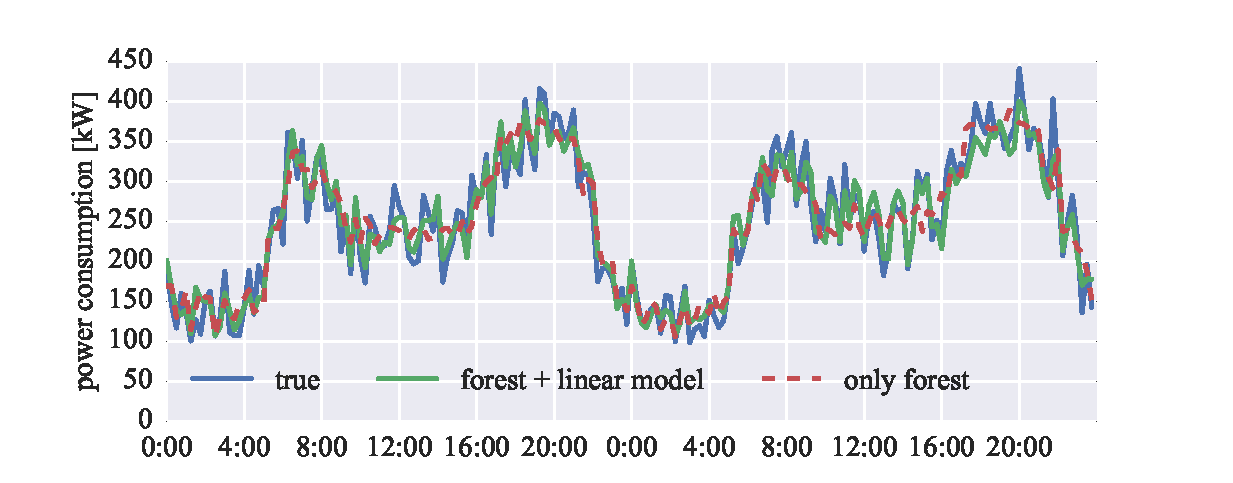
\includegraphics[width=22pc]{figures/eplus_validation.eps}	
	\caption{Model accuracy during training: The prediction made by forest using only $\tX^d$ (red) captures the effect due to disturbances. The linear models in the leaves capture the local effects (green) due to the control inputs $\tX^c$ and improve the model accuracy.}
	\label{F:sepvars}
	\captionsetup{justification=centering}
\end{figure}

\subsection{Power Management}
\label{SS:powermanagement}
Typically, the end customer receives a notification to curtail the power by some fraction. 
In this example on power management, we show how DPC can generate optimal inputs to track a desired power signal within a small allowance while maintaining the zone level thermal comfort. It may not be possible to have the same thermal comfort level in all the zones due to power curtailment, so we choose one zone (for example CEO's office) where the constraints must be met.
This is done by solving the following optimization problem with control variables $\tX^c = [\mathsf{ClgSP},\mathsf{GuestClgSP},\mathsf{KitchenClgSP},\mathsf{SupplyAirSP}, \mathsf{ChwSP}]$ as defined before:
\begin{align}
\begin{aligned}
\text{min } & \ \ \ \ \ \ \ \sum_{j=1}^{N} ({\tP}_{\mathrm{k+j|k}} - \tP_{\mathrm{ref}})^2 +  \lambda\epsilon_j + \nu \delta_j \\
\text{s.~t. } & \ \ \ \ \ \tP_{\mathrm{k+j|k}} =  \hat{\Theta}^T_{\tP_j} [ 1,\tX^c_{\mathrm{k|k}},\dots,\tX^c_{\mathrm{k+j-1|k}} ]^T \\
& \ \ \ \ \ \tT_{\mathrm{k+j|k}} =  \hat{\Theta}^T_{\tT_j} [ 1,\tX^c_{\mathrm{k|k}},\dots,\tX^c_{\mathrm{k+j-1|k}} ]^T \\
& \ \ \ \ \ \ \ \ \ \ \ \ \underline{\tP}-\epsilon_j \leq \tP_{\mathrm{k+j|k}} \leq \bar{\tP} + \epsilon_j\\
& \ \ \ \ \ \ \ \ \ \ \ \ \underline{\tT}-\delta_j \leq \tT_{\mathrm{k+j|k}} \leq \bar{\tT} + \delta_j\\
& \ \ \ \ \ \ \ \ \ \ \ \ \ \ \ \underline{\tX}^c \leq \tX^c_{\mathrm{k+j-1|k}} \leq \bar{\tX}^c\\ 
& \ \ \ \ \ \ \ \ \ \ \ \epsilon_j \geq 0,\delta_j \geq 0, \ j = 1,\dots,N.
\end{aligned}
\label{E:ptrack}
\end{align}

\begin{figure}[h!]
	\subfigure[Optimal inputs calculated by DPC-En. At first, the inputs are changed rapidly because of a significant difference between the desired and the actual power consumption. Then gradual adjustments are made to follow the desired reference.]{
		\label{F:eplus_inputs}
		\centering
		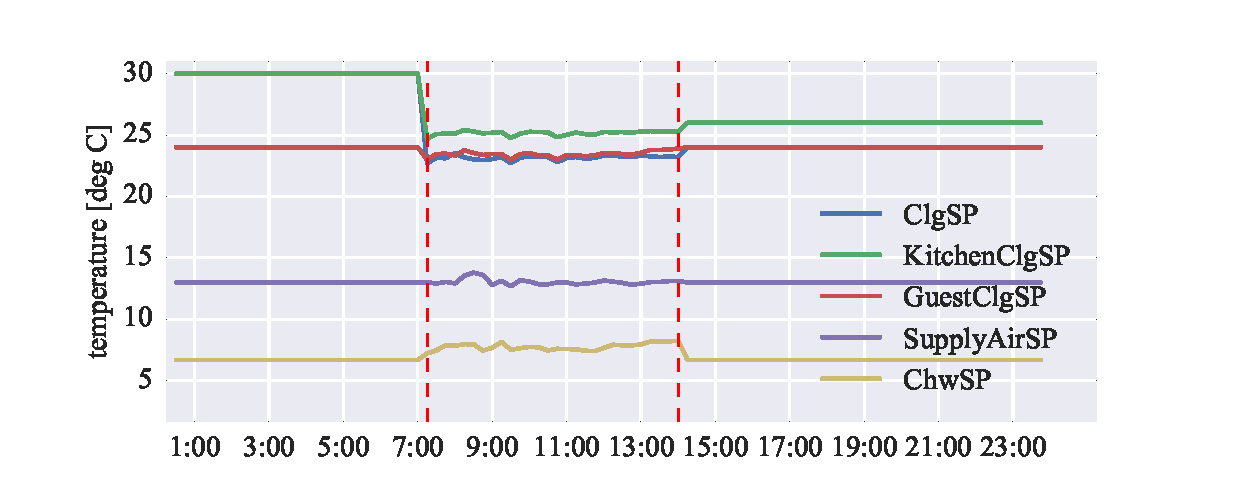
\includegraphics[width=22pc]{figures/eplus_control.eps}
	}
	\subfigure[Power tracking by DPC-En at 1.1 MW: The difference in closed-loop simulation and prediction is due to model mismatch.]{
		\label{F:eplus_power}
		\centering
		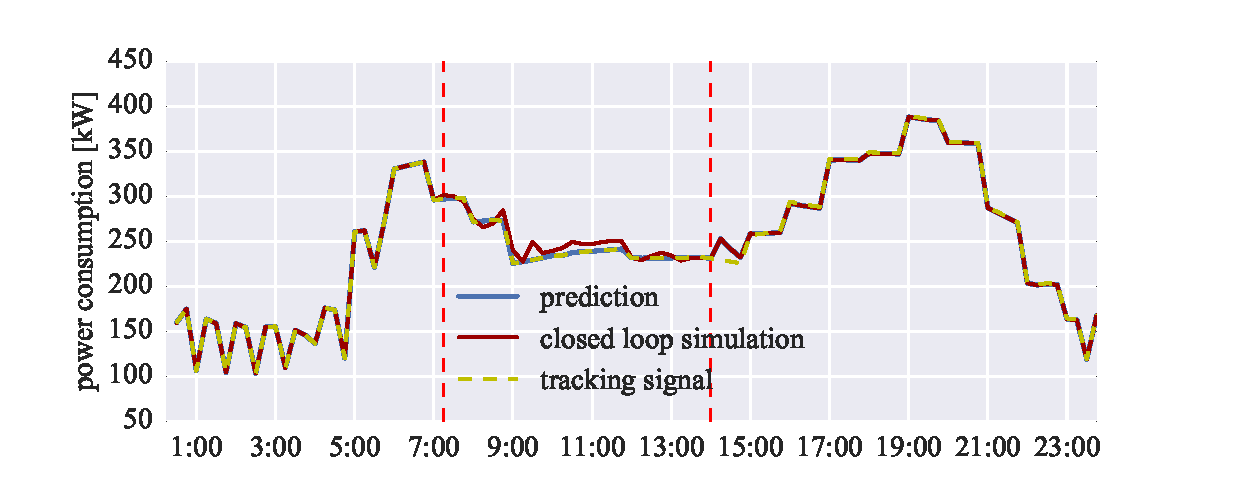
\includegraphics[width=22pc]{figures/eplus_closedloop.eps}
	}
	\caption{Power management using DPC. The controller is active between 7am - 2pm. This region is marked in dashed red lines.}
	\captionsetup{justification=centering}
	\label{F:eplus_track}
\end{figure}

Here, the temperature forests are used to enforce thermal constraints in the zone of interest. The setup of optimization problem is flexible to include even other variables in the cost or the constraints. For example, we are currently looking at including the dynamic pricing of electricity in the cost since the customers can more directly relate to the financial incentives.

The results are shown in Fig.~\ref{F:eplus_track}. 
The DPC controller is active between 7am - 2pm. Before 7am and after 2pm, the building is using a predefined rule-based control strategy.
The optimal control inputs from DPC-En are shown in Fig.~\ref{F:eplus_inputs}. It is observed that, with the optimal inputs generated by DPC, we can track the reference power consumption signal closely. In fact, the average tracking error between 7am - 2pm is 3\%. The difference between the predicted power consumption and that in the closed-loop simulation in Fig.~\ref{F:eplus_power} is due to model mismatch between the EnergyPlus model and the power forest used in the optimization \eqref{E:ptrack}. Due to this inaccuracy, the actual power consumption is on an average 7 kW higher.

Thus, DPC-En successfully tracks a given power reference signal with an average $\sim$ 3\% error for such a complex building which would require several years of efforts to develop a physics based model.




\subsection{Practical Challenges and Future Work}
\label{SS:challenges}
\textit{Data Availability:} The main practical challenge for DPC lies in the availability of data for training and we require answers to questions like how much data (functional testing) is required, and how should the sampling be done? Therefore, the procedure for optimal experiment design, and model improvement with estimation of variance in predictions is one of the main focus of our ongoing work.

\textit{Stability:} While the buildings are inherently stable, many other applications require stability guarantees. In our ongoing work, we are working towards proving asymptotic stability to origin with DPC-RT and DPC-En by using concept of switched LTI systems. This will make DPC useful for systems with faster dynamics.

\textit{Robustness:} Another direction of work is on handling uncertainties in the DPC framework, namely an extension to Scenario DPC to account for the disturbance uncertainty. This will help us in quantifying the robustness of DPC.

